\section{Types of solutions}
\label{solution_types}
Solutions to the hydrodynamic equations~\eqref{eq:hydro_param1}, and~\eqref{eq:hydro_param2} are obtained by integrating away from the position of the bubble wall, $\xi_w$.
There are two relevant external boundary conditions.
To maintain spherical symmetry
\begin{equation}
\lim_{\xi \rightarrow 0} v = 0.
\end{equation}
To maintain causality
\begin{equation}
\lim_{\xi \rightarrow 1} v = 0,
\end{equation}
as no information can propagate faster than light, and we assume the fluid to be stationary until a signal from the expanding bubble arrives.
In addition to these there is one boundary condition for each side of the wall as
\begin{equation}
\lim_{\xi \rightarrow \xi_w^\pm = v_w \pm \delta, \ \delta \rightarrow 0} v = v_\pm = \mu (\xi_w, \tilde{v}_\pm),
\end{equation}

There are two ways to satisfy these conditions.
We can either start at $v=0$, or from a region where $\xi > c_{s-}(w)$ and $\mu(\xi,v) > c_{s-}(w)$, and therefore $\frac{dv}{d\xi} > 0$,
and integrating backwards in $\xi$ over a route where $\mu(\xi,v) > c_{s-}(w)$ is satisfied.
The other way to reach $v=0$ is by a discontinuity, i.e. a shock.
This leads to two classes of solutions.
Another way to see that there are two classes of solutions is by noting
that the equations \eqref{eq:v_tilde_plus} and \eqref{eq:v_tilde_minus} have two branches.
These solutions are classified in table \ref{table:solution_types}.

\begin{table}[ht!]
\small
\caption{Types of solutions to the hydrodynamic equations}
\begin{tabular}{r|c|c}
                & Detonations            & Deflagrations \\
                & $p_+ < p_-, \tilde{v}_+ > \tilde{v}_-$ & $p_+ > p_-, \tilde{v}_+ < \tilde{v}_-$ \\ \hline
Weak            & $\tilde{v}_+ > c_{s+}(w_+), \ \tilde{v}_- > c_{s-}(w_-)$ & $\tilde{v}_+ < c_{s+}(w_+), \ \tilde{v}_- < c_{s-}(w_-)$ \\
Chapman-Jouguet & $\tilde{v}_+ > c_{s+}(w_+), \ \tilde{v}_- = c_{s-}(w_-)$ & $\tilde{v}_+ < c_{s+}(w_+), \ \tilde{v}_- = c_{s-}(w_-)$ \\
Strong          & {\color{gray} $\tilde{v}_+ > c_{s+}(w_+), \ \tilde{v}_- < c_{s-}(w_-)$} & {\color{gray} $\tilde{v}_+ < c_{s+}(w_+), \ \tilde{v}_- > c_{s-}(w_-)$} \\
\end{tabular}
\label{table:solution_types}
\end{table}

The solutions with $\tilde{v}_+ > \tilde{v}_-$ are known as detonations.
% In this case there is no way for the front to influence the fluid ahead,
% and the outermost front is a shock.
Detonations are further characterised by the scale of their $\tilde{v}_-$.
In weak detonations $\tilde{v}_- > c_{s-}(w_-)$.%
\footnote{The note in \cite[p. 265]{rezzolla_relativistic_2013} that weak detonations are not possible in an exothermic reaction does not apply to cosmological phase transitions, since in them the number of particles is not conserved.}
Correspondingly, detonations with $\tilde{v}_- < c_{s-}(w_-)$ are known as strong detonations.
However, they are unstable and will naturally evolve into the third class of detonations,
the Chapman-Jouguet detonations, for which $\tilde{v}_- = c_{s-}(w_-)$.
\cite[p. 279]{rezzolla_relativistic_2013}
Since we are investigating a self-similar bubble that has already evolved for some time,
the most of our detonations are weak detonations,
and those at the detonation-hybrid boundary are Chapman-Jouguet detonations.
In detonations the shock and phase boundary fronts are unified to a single front.
\cite{kurki-suonio_supersonic_1995}

The solutions where $\tilde{v}_+ < \tilde{v}_-$ are known as deflagrations.
In them the phase front can influence the fluid ahead, and the wall is preceded by an accelerating fluid and a shock.
Strong deflagrations are not possible in an exothermic reaction.
\cite[p. 267]{rezzolla_relativistic_2013}
Therefore, only weak and Chapman-Jouguet deflagrations are possible.
In weak detonations the fluid inside the phase boundary is still, and the preceding shock is weak and
known as the precompression front.
\cite{rezzolla_relativistic_2013}

The third class of solutions are the supersonic deflagrations, also known as hybrids.
They consist of a Chapman-Jouguet deflagration followed by a detonation-like rarefaction wave.
In hybrids the wall speed exceeds the speed of sound in the broken phase $c_{s-}$,
and the fluid is moving inside the phase boundary as well, as in a detonation.
\cites{kurki-suonio_supersonic_1995}[p. 37]{lecture_notes}[p. 35]{hindmarsh_gw_pt_2019}
The three solution types: subsonic deflagrations, supersonic deflagrations aka. hybrids and detonations are illustrated in figure \ref{fig:solution_types}.

\begin{figure}[ht!]
\centering
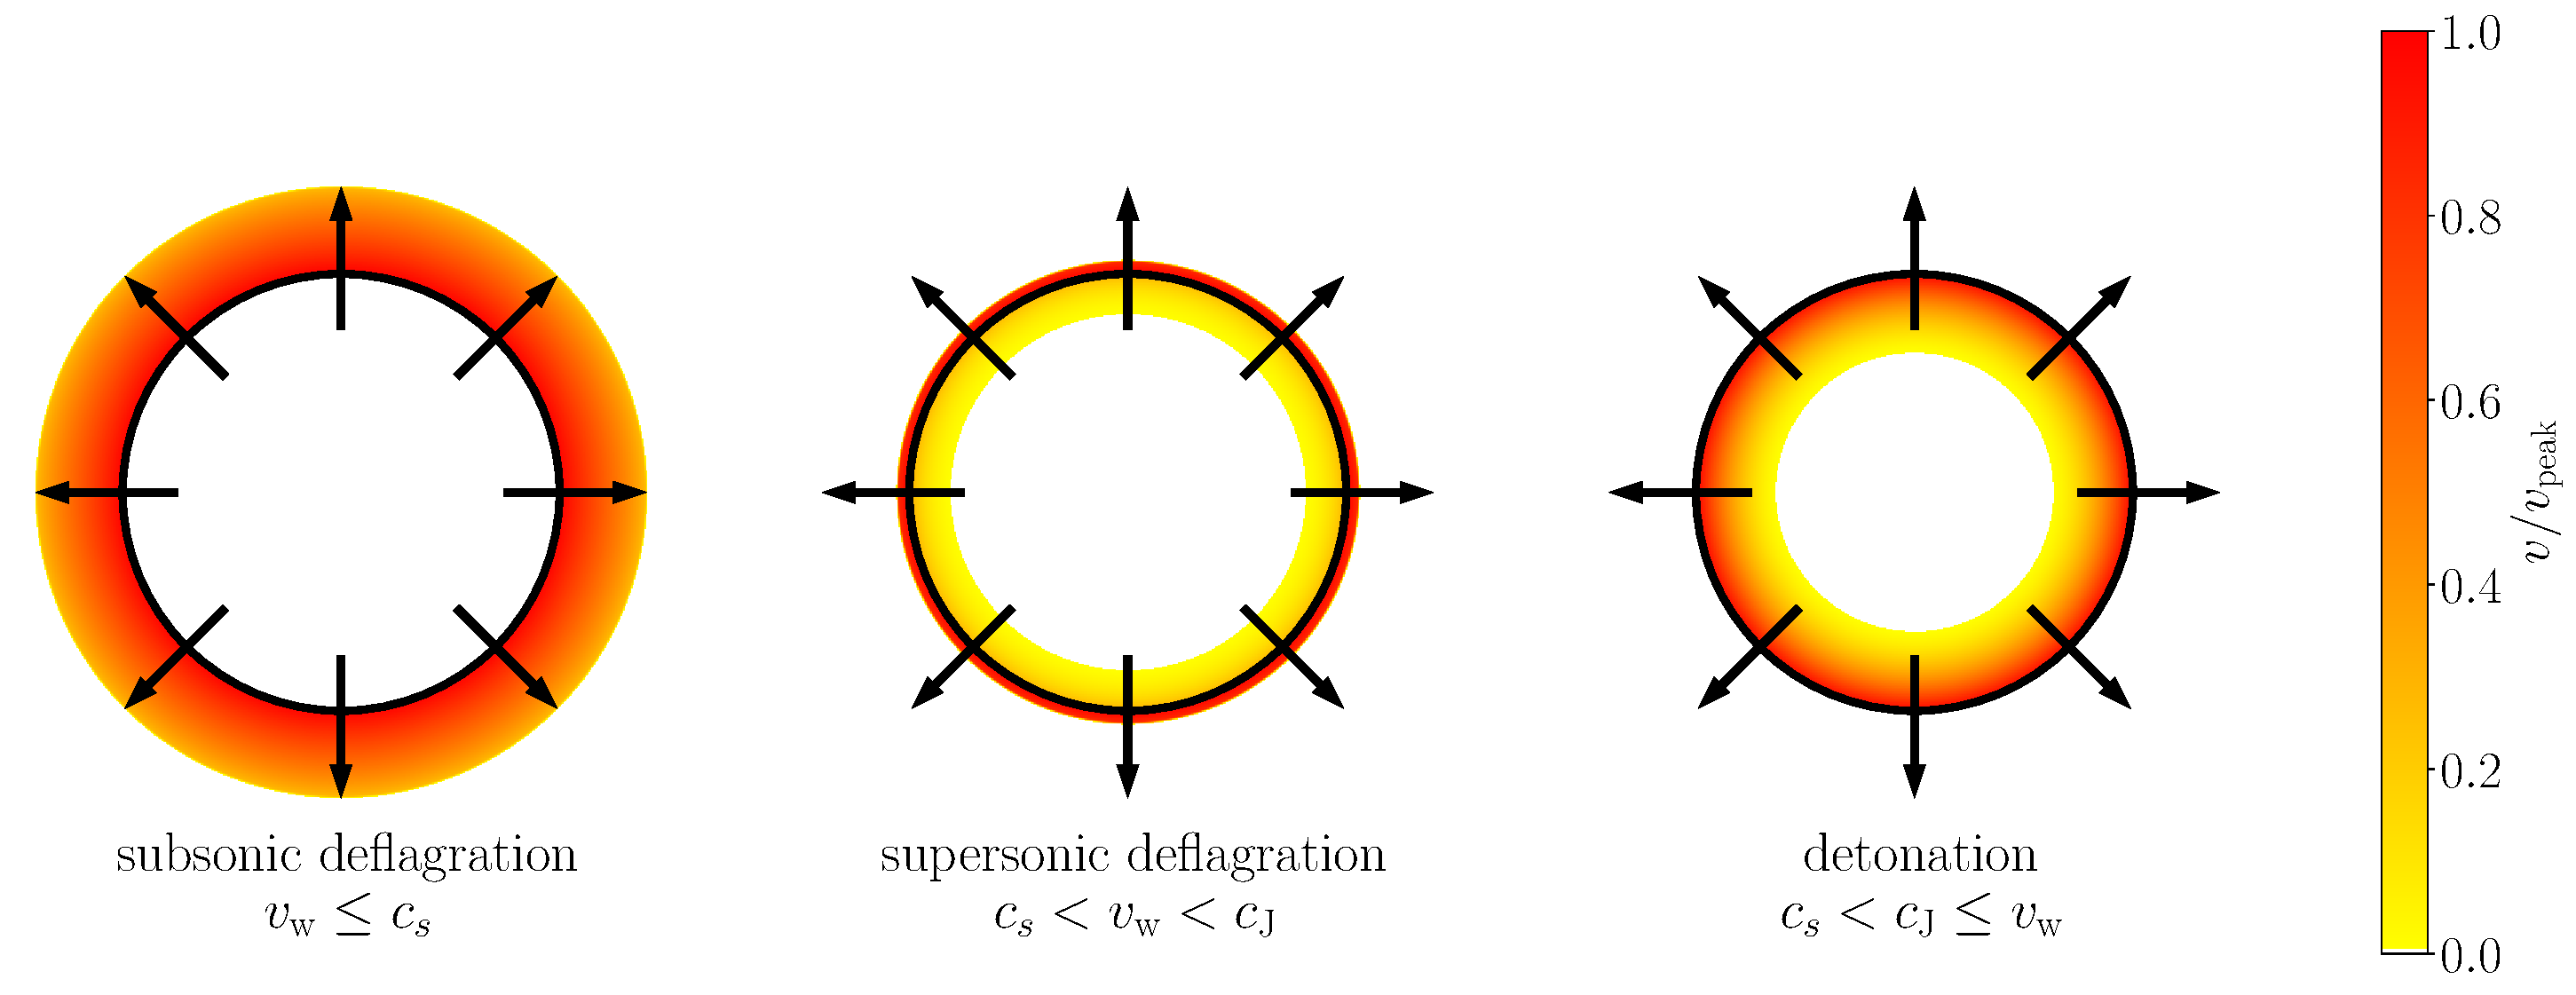
\includegraphics[width=\textwidth]{fig/relativistic_combustion.pdf}
\caption{Three different types of relativistic combustion. Generated with PTtools. See also \cites[fig. 14]{lecture_notes}[fig. 14]{mazumdar_review_2019}.}
\label{fig:solution_types}
\end{figure}


\clearpage
\FloatBarrier
\subsection{Speed limits}
The observables of a physical system must be real, including $\tilde{v}_+$ and $\tilde{v}_-$.
Therefore the expressions in the square roots of eq. \eqref{eq:v_tilde_plus} and \eqref{eq:v_tilde_minus} must be real.
By simplifying the expression in the square root of eq. \eqref{eq:v_tilde_plus} we see that the square root is real $\forall \alpha_+ \geq 0$,
but setting the square root in eq. \eqref{eq:v_tilde_minus} to zero gives a limit for $\tilde{v}_+$ as
\begin{equation}
\tilde{v}_+ = \frac{1}{\sqrt{3}} \left( \frac{1 \pm \sqrt{2 \alpha_+ + 3 \alpha_+^2}}{1 + \alpha_+} \right).
\label{eq:v_tilde_plus_limit}
\end{equation}
The positive sign is the lower limit for detonations, and the negative sign is the upper limit for deflagrations.%
\footnote{This is the same equation as in \cites[eq. 7.34]{lecture_notes}[eq. B.19]{hindmarsh_gw_pt_2019},
but in those articles there is a typo due to which a factor of 2 is missing from the expression.}

Inserting this value to the equation \eqref{eq:v_tilde_minus} and simplifying the expression with the knowledge that the square root is now zero
we get that
\begin{equation}
\tilde{v}_- = \frac{1}{\sqrt{3}}.
\label{eq:v_tilde_minus_limit}
\end{equation}
This is the lower limit for detonations, and the upper limit for deflagrations.

The Chapman-Jouguet speed is defined as
\begin{equation}
\tilde{v}_+=v_{CJ} \Leftrightarrow \tilde{v}_- = c_{s-}(w_-).
\label{eq:chapman_jouguet}
\end{equation}
Starting from section \eqref{bag_model} we will see that for some models the speed limit set by the Chapman-Jouguet speed of \eqref{eq:chapman_jouguet}
and the condition of \eqref{eq:v_tilde_minus_limit} that the observables are real are equivalent,
but in general this is not the case.

Now we have the necessary knowledge to classify the different regions of fig. \eqref{fig:vplus_vminus}.
If the speeds of sound are equivalent to $\frac{1}{\sqrt{3}}$,
we can have only weak and Chapman-Jouguet detonations and deflagrations.
When the speed of sound in the broken phase $c_{s-}(w_-) < \frac{1}{\sqrt{3}}$,
we could have a strong deflagration where $c_{s-}(w_-) < \tilde{v}_- < \frac{1}{\sqrt{3}}$,
but this is ruled out by the fact that the phase transition is exothermic.
Correspondingly, when $c_{s-}(w_-) > \frac{1}{\sqrt{3}}$,
we can have a strong detonation where $\frac{1}{\sqrt{3}} < \tilde{v}_-(w_-, \phi_-) < c_{s-}(w_-)$,
but as previously discussed, a strong detonation is unstable and will evolve into a Chapman-Jouguet detonation.
Since for Chapman-Jouguet detonations $v_w = \tilde{v}_+ > \tilde{v}_-$,
the Chapman-Jouguet speed is the lower speed limit for detonations that have been evolving for a sufficiently long time.
